%  !TeX  root  =  user_guide.tex

\section{Plugin Spatial Query}\label{sec:spatial_query}

% when the revision of a section has been finalized, 
% comment out the following line:
% \updatedisclaimer

Il plugin \toolbtntwo{spatialquery}{Spatial Query} permette di definire una query 
spaziale di selezione in un layer target con riferimento ad un altro layer. La funzionalità 
si basa sulla libreria GEOS. 

Gli operatori spaziali sono:

\begin{itemize}[label=--]
\item Attraversa
\item Interseca
\item È disgiunto
\item Tocca
\item Contenuto
\end{itemize}

Per i layer di poligoni gli operatori 'Tocca' e 'Attraversa' non sono disponibili.

\minisec{Come usare il plugin}

L'esempio che segue mostra come individuare le regioni dell'Alaska che contengono degli aeroporti:

\begin{enumerate}
  \item Avviare QGIS e caricare i layer vettoriali regions.shp e airports.shp. 
  \item Caricare il plugin Spatial Query nel Gestore plugin (Sezione 
  \ref{sec:load_core_plugin}) e cliccare sull'icona \toolbtntwo{spatialquery}{Spatial Query}    
  nella barra dei strumenti plugin: la finestra di dialogo Interrogazione spaziale è mostrata nella Figura \ref{fig:spatialquerysample}.
  \item Selezionare regions come sorgente degli oggetti e airports come riferimento.
  \item Selezionare 'Contiene' come operatore e cliccare su \button{Apply}.
\end{enumerate}

A questo punto appare un riquadro che elenca gli ID degli elementi che soddisfano la query; si hanno diverse opzioni 
per utilizzare i risultati:

\begin{itemize}[label=--]
\item Cliccare su \toolbtntwo{selectesubsetlayer}{Crea layer con lista di oggetti}
\item Selezionare un elemento dalla lista e cliccare \toolbtntwo{selectcreatelayer}{Crea layer con selezionato}
\item Selezionare \button{Rimuovi dalla sessione corrente} nel campo 'E usa il risultato per'.
\item Opzionalmente è possibile selezionare le caselle di controllo \checkbox{Zoom all'oggetto} e \checkbox{Messaggi di log}.
\end{itemize}

\begin{figure}[ht]
   \centering
   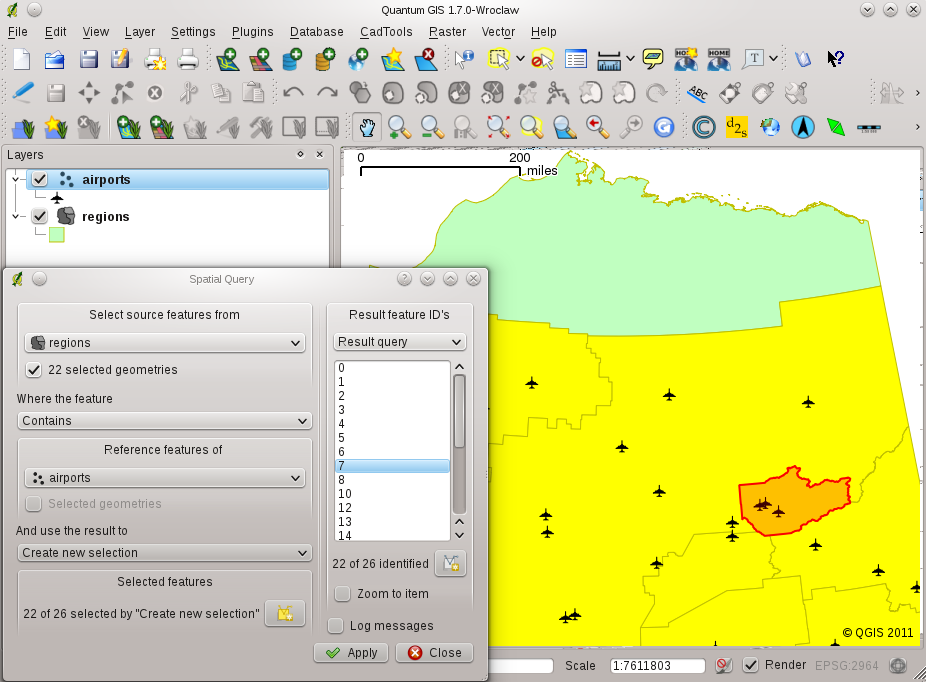
\includegraphics[clip=true, width=14cm]{spatial_query_sample}
   \caption{Interrogazione spaziale - Regioni che contengono aeroporti \wincaption}
   \label{fig:spatialquerysample}
\end{figure}

\FloatBarrier

